
\RequirePackage{lineno}
\documentclass[11pt]{article}
%
\usepackage{graphicx}  % Include figure files
\usepackage{dcolumn}   % Align table columns on decimal point
\usepackage{bm}        % bold math
\usepackage{amssymb}   % for math
\usepackage{multirow}
\usepackage{lineno}
\usepackage{amsmath}
\usepackage{xcolor}
\usepackage{sectsty}
\usepackage{indentfirst}
\usepackage{lipsum}
\usepackage{csquotes}
\sectionfont{\fontsize{12}{15}\selectfont}

%--------
%\usepackage{doublespace}

%
\begin{document}

\title{{ \large*** Draft *** \\ (A New Proposal to Jefferson Lab PAC 48)} \\
%\vspace{1em}
\textbf{ \large Two-Photon Exchange Contribution in Elastic $e-n$ Scattering}}
\author{\small authors (TBD)}
\date{\small \today}
\maketitle 
\begin{abstract}
We propose make a high precision measurement of the two-photon exchange contribution (TPE) in elastic electron-neutron scattering at a four-momentum transfer $Q^2$ = 4.5 (GeV/c)$^2$. While significant efforts to study the two-photon-exchange have centered around elastic electron-proton scattering, the impact of TPE on neutron form factors was never examined experimentally. The proposed experiment will provide the very first assessment of the two-photon exchange in electron-neutron scattering, which will be very useful for understanding hadronic physics. \par
The proposed experiment would be performed in Hall A using the BigBite (BB) spectrometer to detect the scattered electrons and the Super-BigBite (SBS) to detect protons and neutrons. The experiment should run concurrently with the E12-09-019 $G_M^n$ and E12-17-004 $G_E^n$-Recoil experiments, which are approved to run early 2021. The experimental setup of this proposed experiment should be identical to that of E12-09-019 experiment. \par
The \enquote{ratio} method will be used to extract the electric form factor of the neutron $G_E^n$ by scattering unpolarized electrons from deuterium quasi-elastically at $Q^2$ = 4.5 (GeV/c)$^2$. In the proposed method, systematic errors are greatly reduced compared to the use of the traditional Rosenbluth method. Several experiments have used the ratio method to extract the neutron magnetic form factor in the past years. The same method can be used to extract the neutron electric form factor even with less stringent requirements on the knowledge of the absolute neutron detection efficiency. \par
% We propose to add a kinematic point at $Q^2$ = 4.5 (GeV/c)$^2$ with high $\epsilon$ value, which will be used along with one of E12-09-019 kinematic points to extract the form factors ratio $g=G_E/G_M$ using Rosenbluth method. 
\end{abstract}
\tableofcontents
\linenumbers
\section{Introduction}\label{sec:sec1}

In 1950's, a series of experiments performed by Hofstadter \cite{hof} revealed that the nucleons have a substructure (would be called later quarks) confirming Rosenbluth theory \cite{rosen}. 
In the Born approximation, where the interaction between the electron and the nucleon occurs $via$ an exchange of a single virtual photon, the unpolarized $e-N$ elastic cross section can be expressed in terms of a nucleon magnetic, $G_M$, and electric, $G_E$, form factors. The form factors describe the deviation from a point-like behavior of the nucleon:  

\begin{equation}\label{eq:1}
\bigg(\cfrac{d\sigma}{ d\Omega}\bigg)_{eN\rightarrow eN}  = \cfrac{\tau \sigma_{Mott}}{\epsilon(1+\tau)}\;\; \big[G^{2}_{M}(Q^2) + \cfrac{\epsilon}{\tau} \; G^{2}_{E}(Q^2)\big] \;\; ,
\end{equation}
 where $E$ and $E'$ are the incident and scattered beam energies respectively, $\theta$ is the scattering angle, $\tau \equiv -q^{2}/4M^{2}$,  with $-q^2 \equiv Q^2 = 4EE'\sin{(\theta/2)}$ being the squared four momentum transfer, $M$ is the proton mass, and $\epsilon = \big[ 1 + 2(1+\tau) \tan^2{(\theta/2)} \big]^{-1}$ is the longitudinal polarization of the virtual photon.\par
 \begin{figure}[h]
\begin{center}
  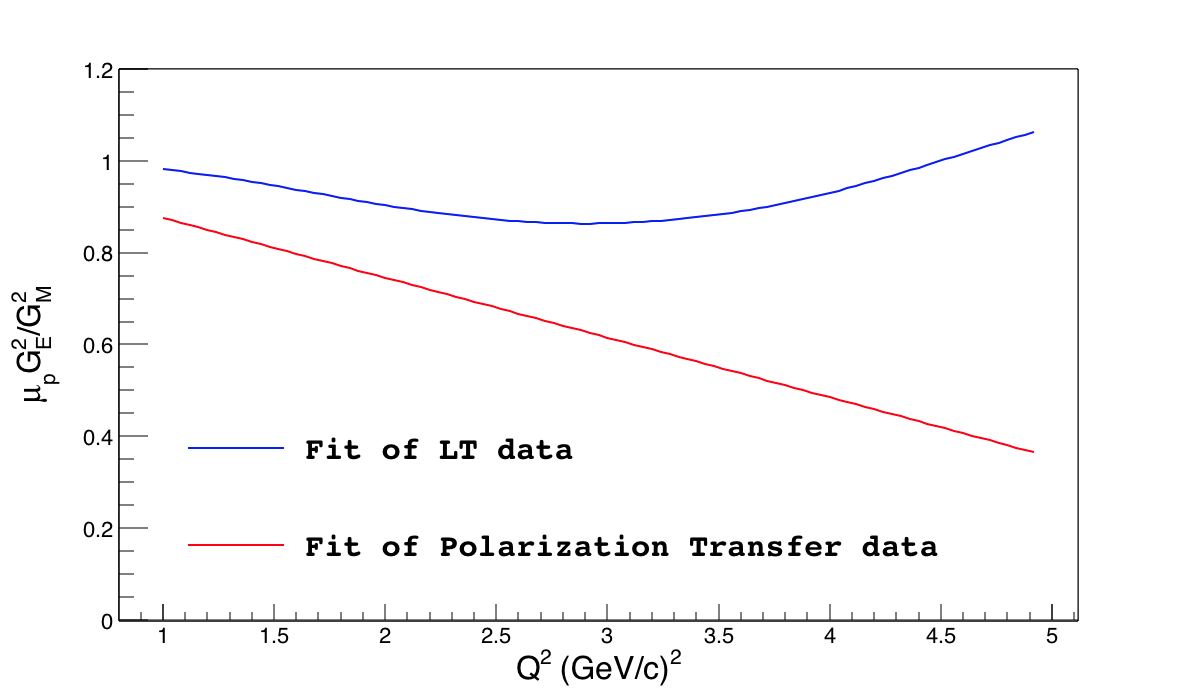
\includegraphics[width=12cm,height=8cm]{TPE.png}
  \caption{(Blue line) Linear fit based on global analysis of Rosenbluth results \cite{john}. (Red Line) Linear fit  to polarization transfer observables \cite{gayou}. }
  \label{fig:TPE}
  \end{center}
\end{figure}
The nucleon electromagnetic form factors can reveal a lot of information about the nucleon internal structure, as well as the quark distribution. The form factors depend only on the square of the four-momentum transfer carried by the photon, $Q^2$. In the limit of large $Q^2$, pQCD provides well-founded predictions for the $Q^2$-dependance of the form factors and their ratio. However, it was found later \cite{qcd, qcd2} that the proton electric and magnetic form factors behave differently starting at $Q^2 \approx$ 1 (GeV/c)$^2$, and pQCD is not applicable up to $Q^2 = $10 (GeV/c)$^2$. Since protons and neutrons share many similar properties, it is expected that the neutron form factors will show the same $Q^2$-dependance as the proton.
\par
Experimentally, the nucleon form factors can be measured using one of two techniques: polarization transfer technique and Rosenbluth technique. The polarization method examines the polarization transfer to the recoiling nucleon and determine the resulting azimuthal asymmetry distribution using a polarimeter. While in the Rosenbluth method, the electric and magnetic from factors can be separated by making two or more measurements with different $\epsilon$ values ($i.e.$ different beam energies and angles), but with same $Q^2$ value. Applying Rosenbluth technique requires an accurate measurement of the cross section and suffers from large systematic uncertainties arising from several factors. For instance, an accurate knowledge of the neutron detector efficiency is required. When comparing the values of $G_E^p/G_M^p$ obtained from both techniques, a significant discrepancy (see Fig.\ref{fig:TPE}) over a wide range of $Q^2$ was observed. Such discrepancy implies uncertainties in our understanding of the nucleon substructure. Many efforts were made in order to provide legitimate explanation, and it is believed that the inconsistency is due to missing corrections. The radiation corrections are well understood for the unpolarized scattering and very small for the polarized observables. On the other hand, not all terms of the two-photon exchange corrections were taken into account, which are potentially important at large $Q^2$. In Born approximation, the reduced cross section depends linearly on $\epsilon$, and any deviation from this linearity is an indication of a missing correction. Therefore, studying the $\epsilon$ dependence of the reduced cross section provides a clean measurement of the TPE cotributions . At large $Q^2$ values, above 3-4 (GeV/c)$^2$, the form factor $G_E$ is very small and any $\epsilon$ dependence must likely come from TPE contribution.  
\par
There was significant amount of effort put into studying the impact of TPE on the proton form factors \cite{john, gayou}, however, no such study was performed for neutron electric form factor. \textbf{\small We propose to make the first assessment of the two-photon-exchange contribution on the neutron form factor (nTPE). The results of nTPE will possibly add a new dimension to our understanding of hadronic physics}.

\section{Technique}
The neutron form factors are challenging to be measured experimentally mainly because there is no free neutron target. However, since the deuterium is a loosely coupled system, it can be viewed as the sum of a proton target and a neutron target at high $Q^2$. In fact, quasi-elastic scattering from deuterium has been used to extract the neutron magnetic form factor, $G_M^n$, at high $Q^2$ for decades \cite{QES1,QES2,QES3,QES4}. However, the proton cross section needs to be subtracted by applying a single-arm quasi-elastic electron-proton scattering. This \enquote{proton-subtraction} technique suffers from big systematic errors. 
\par
Durand \cite{durand} proposed the so-called \enquote{ratio-method} - which will be discussed in detail in a later section- to measure the neutron form factors. In this method, many of the systematic errors that plague other methods will cancel out. Several experiments  \cite{bonn, mainz, jlab} have applied the ratio-method to determine the neutron magnetic form factor. We propose to use the same method to extract the neutron electric form factor, $G_E^n$, with even less constraints on the knowledge of the absolute efficiency of the neutron detector. Data will be collected from quasi-elastic electron scattering from deuteron $D(e,e'n)p$. A complementary $D(e,e'p)n$ data will be taken to calibrate the experiment. 
As mentioned in Sec. \ref{sec:sec1}, applying Rosenbluth technique to measure $G_E^n$ requires accurate measurement of the cross section and suffers from large systematic uncertainties. To overcome this issue, we propose to extract the value of $G_E^n$ from the measured ratio of quasi-elastic e-n to e-p scattering from a deuteron target as follows: 

\begin{equation}
R_{observed} = \cfrac{\frac{d\sigma}{d\Omega} |_{D(e,e'n)p}}{\frac{d\sigma}{d\Omega} |_{D(e,e'p)n}} \;\; .
\end{equation}
$R_{observed}$ needs to be corrected to extract the ratio of e-n/e-p scattering from free nucleons:

\begin{equation}\label{eq:3}
R_{corr} = f_{corr} \times R_{observed} \;\; ,
\end{equation}
where the correction factor $f_{corr}$ includes all the necessary corrections such as the radiative corrections and nuclear corrections.
Using Eq.\ref{eq:1}, $R_{corr}$ can be written as: 

\begin{equation}
R_{corr} = \cfrac{ \cfrac{\sigma_{Mott}^n}{(1+\tau_n)}\;\; \big[\cfrac{\tau_n}{\epsilon_n} \;G^{2}_{M,n}(Q^2) +  G^{2}_{E,n}(Q^2)\big]}{ \cfrac{\sigma_{Mott}^p}{(1+\tau_p)}\;\; \big[\cfrac{\tau_p}{\epsilon_p} \;G^{2}_{M,p}(Q^2) +  G^{2}_{E,p}(Q^2)\big]} \;\; .
\end{equation}

Solving Eqs.\ref{eq:1} and \ref{eq:3} for $G_E^n$ we get: 

\begin{equation}
G_E^n = \sqrt{R_{corr}\bigg(\cfrac{ \sigma_{Mott}^n}{ \sigma_{Mott}^p}\bigg) \bigg(\cfrac{1+\tau_n}{1+\tau_p}\bigg)\big[\cfrac{\tau_p}{\epsilon_p} \; G^{2}_{M,p}(Q^2) + G^{2}_{E,p}(Q^2)\big] - \cfrac{\tau_n}{\epsilon_n}\; G_{M,n}^2  }
\end{equation}

One can write the electromagnetic form factors in terms of the total form factor $F^2$, where:

\begin{equation}
F^2 = \cfrac{1}{\epsilon (1 + \tau)} \; [\epsilon G_E^2 + \tau G_M^2] \;\; .
\end{equation}

The total form factor is calculated from the event rates corrected by the experiment parameters as following: 

\begin{equation}
F^2 = \cfrac{ N_{\text{events}}}{I_{\text{beam}} \cdot \rho_{\text{target}} \cdot t_{DAQ} \cdot \sigma_{Mott} \cdot \Omega_e \cdot \eta_e} \;\; ,
\end{equation}
where $I_{\text{beam}}$ is the beam current, $\rho_{\text{target}}$ is the target density, $t_{DAQ}$ is the data taking time, $\Omega_e$ is the detector solid angle, and $\eta_e$ is the detection efficiency. Each parameter is known with limited accuracy, leading to higher systematics. To overcome this issue, one can apply the Rosenbluth technique to obtain the ratio $g = G_E/G_M$ from $F^2$. By making two measurements at the same $Q^2$ but with different $\epsilon$ value, the ratio $g$ can be calculated using the following equation \cite{bogdan}:

\begin{equation}
g^2 = \tau \cdot \cfrac{F_{\epsilon_1}^2 \epsilon_2^{-1}- F_{\epsilon_2}^2 \epsilon_1^{-1}}{F_{\epsilon_2}^2  - F_{\epsilon_1}^2 } \;\; ,
\end{equation} 
The uncertainty of $g$, which increases with $Q^2$, can be estimated using the equation:

\begin{equation}
\sigma (g^2) \approx \cfrac{\sigma (F_{\epsilon}^2)}{F_{\epsilon}^2} \cfrac{\sqrt{2} \cdot \tau}{\epsilon_1 - \epsilon_2} \;\; ,
\end{equation}
where the uncertainties in $\epsilon$ and $\tau$ are neglected. Several factors cancel out when calculating the ratio $g$ such as the target density and detection efficiency. However, accurate determination of the beam energy, the detector solid angle and the scattering angle is still crucial for this experiment. \par
The value of $g_n$ can be obtained from the ratio $F_{\epsilon_2}^n/F_{\epsilon_1}^n$  as:

\begin{equation}
\bigg(\cfrac{F_{\epsilon_2}^n}{F_{\epsilon_1}^n}\bigg)^2 = \bigg(\cfrac{F_{\epsilon_2}^p}{F_{\epsilon_1}^p}\bigg)^2 \cdot \cfrac{N_2^{e,e'n}}{N_1^{e,e'n}} \cdot \cfrac{N_1^{e,e'p}}{N_2^{e,e'p}} \cdot \cfrac{\Omega_{\epsilon_2}^n}{\Omega_{\epsilon_1}^n}  \cdot \cfrac{\Omega_{\epsilon_1}^p}{\Omega_{\epsilon_2}^p} \cdot \cfrac{\eta_{\epsilon_2}^n}{\eta_{\epsilon_1}^n}  \cdot \cfrac{\eta_{\epsilon_1}^p}{\eta_{\epsilon_2}^p} \;\; .
\end{equation}
 Several parameters such as the beam current, the electron-arm solid angle and efficiency, the Mott cross section, the data taking time, and the target parameters all cancel out from the final ratio of the form factors at two different values of $\epsilon$. The remaining parameters are the neutron/proton detector solid angle $\Omega$ and efficiency $\eta$, whose variations for different $\epsilon$ need to be controlled.
\section{Proposed Kinematics}
We propose to use the same experimental setup of E12-09-019 experiment. We will add a kinematic point at $Q^2$ = 4.5 (GeV/c)$^2$, but with a higher $\epsilon$ value. This additional point along with the data point of E12-09-019 experiment will allow us to perform Rosenbluth technique and obtain $G_E^n$ value. Table \ref{tab:table1} displays the kinematic setting of the proposed experiment. 
\begin{center}
\begin{table}[h]
\begin{tabular}{|>{\centering}m{0.3in} |>{\centering}m{0.55in}|>{\centering}m{0.4in}| >{\centering}m{0.4in}| >{\centering}m{0.45in}|>{\centering}m{0.45in}|>{\centering}m{0.4in}|>{\centering}m{0.4in}|>{\centering\arraybackslash}m{0.4in}|}
\hline
\small{Point} & $Q\textsuperscript{2}$  & E & E$'$  & $\theta_{BB}$ & $\theta_{SBS}$ & $\epsilon$ &$\Delta \sigma$ & $\Delta TPE$\\
& (GeV/c)$^2$ & (GeV) & (GeV)  & degrees & degrees   &  & (\%)& (\%) \\
\hline
\textcolor{blue}
 1&\textcolor{blue} {4.5} & \textcolor{blue}{4.4} & \textcolor{blue}{2.0} & \textcolor{blue}{41.88}  & \textcolor{blue}{24.67} & \textcolor{blue}{0.599} & & \\
\hline
2 & 4.5  &  6.6  &  4.2  & 23.23  &  31.2  &  0.838 & & \\
\hline
\end{tabular} 
\caption{Kinematic settings of the proposed experiment. The blue row is a kinematic point of E12-09-019 experiment}
\label{tab:table1}
\end{table}
\end{center}

\section{Apparatus} 
A major goal of the experiment is the study any nonlinearities in the $\epsilon$ dependance using the ratio method. Such method depends on the detection of both scattered neutrons and protons. We propose to run concurrently with E12-09-019 experiment that is approved to run in Hall A. Our experiment will use the same apparatus of E12-09-019. The BigBite spectrometer will be used to detect electrons, while the Super-BigBite spectrometer will be used to detect neutrons and protons. The 10 cm long liquid deuterium target will be used along with the liquid hydrogen for calibration. The experimental setup (e.g. detectors, triggers, targets..etc) is described in detailed \cite{gmp}. 
\section{Systematic Errors}
\section{Beam Time Request}


\begin{thebibliography}{9}
\bibitem{hof}
R. Hofstadter, Rev. Mod. Phys. 28, 214 (1956)

\bibitem{rosen}
M. N. Rosenbluth, Phys. Rev. 79, 615 (1950)


\bibitem{qcd}
M. Jones \emph{et al.}, Phys. Rev. Lett. 84, 1398 (2000).

\bibitem{qcd2}
O. Gayou \emph{et al.}, Phys. Rev. Lett. 88, 092301 (2002).

\bibitem{john}
J. Arrington, Phys. Rev. C 69, 022201(R) (2004).

\bibitem{gayou}
O. Gayou et al., Phys. Rev. Lett. 88, 092301 (2002)
%\bibitem{christy}
%M. E. Christy \emph{et al.}, Phys. Rev. C 70, 015206 (2004).

%\bibitem{john}
%J. Arrington, Phys. Rev. C 69, 022201(R) (2004).
\bibitem{QES1}
E.B. Hughes et al., Phys. Rev. 139, B458 (1965).

\bibitem{QES2}
R.G. Arnold et al., Phys. Rev. Lett. 61, 806 (1988).

\bibitem{QES3}
 E.E.W. Bruins et al., Phys. Rev. Lett. 75, 21 (1995).

\bibitem{durand}
L. Durand, Phys. Rev. 115, 1020 (1959).

%\bibitem{john2} 
%John Arrington et al 2011 J. Phys.: Conf. Ser. 299 012002. 

\bibitem{bonn}
E.E.W. Bruins \emph{et al.}, Phys. Rev. Lett. 75, 21 (1995).

\bibitem{mainz}
G. Kubon \emph{et al.}, Phys. Lett. B524, 26 (2002).

\bibitem{jlab}
W. Brooks  \emph{et. al.}, JLab experiment E94-017.

\bibitem{bogdan}
B. Wojtsekhowski, arXiv:1706.02747 [physics.ins-det], report at High-t, 2002.

\bibitem{gmp}
B. Quinn \emph{et. al.}, Jefferson Lab experiment E12-09-019
\end{thebibliography}
\end{document}

  








